\section{Sensor Nodes}

\begin{figure}[ht!]
   \centering
   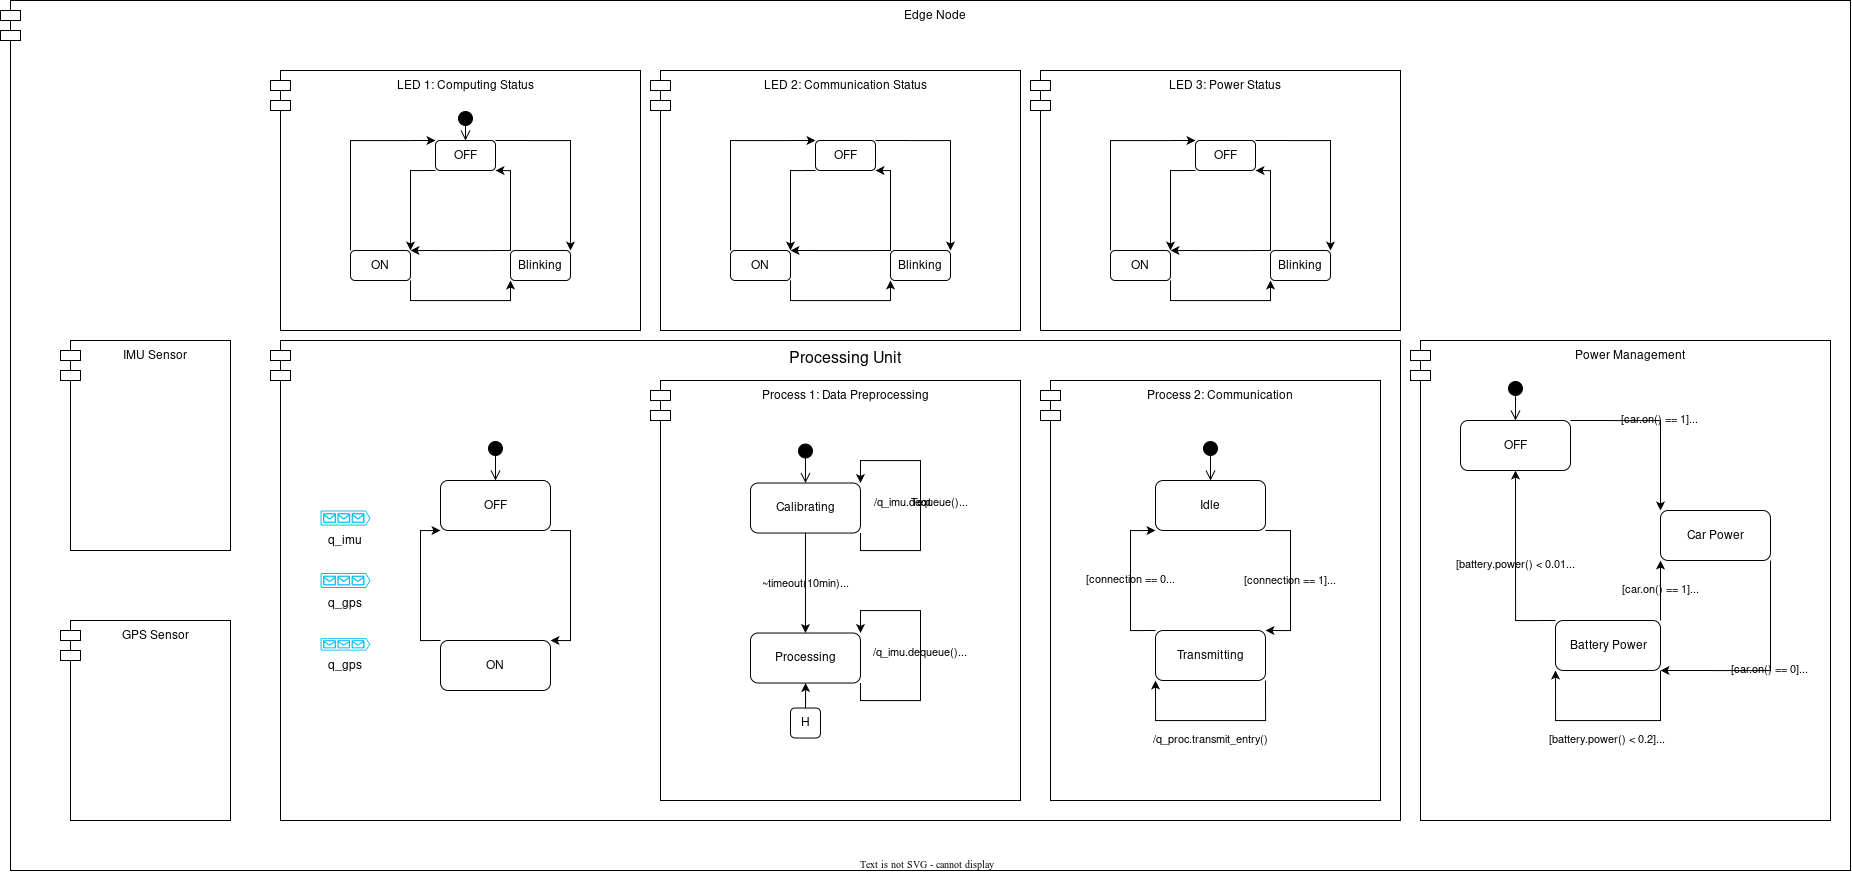
\includegraphics[width=\textwidth]{../../assets/diagrams/edge_node_rtuml/edge_node_rtuml.png}
   \hfill
   \caption{RT-UML of a Sensor Node}
   \label{fig:rt_uml_sensor_node}
\end{figure}

\begin{enumerate}
    \item \textbf{Cost Restriction per node}: ~100 CHF  \\
       As the number of vehicles the nodes will be high, th cost per node needs to be as small possible. To keep cost of installation and parts low, one single node/sensor package will be installed inside the vehicle.
    
    \item \textbf{Quantify felt RoadState}:
       The node is idealy placed centraly in the car, above one of the axles and mounted securely to the chassis to minimize errors.
       Roadstate will be quantified in a range of 0 (very good) to 244 (very bad) with a value of 255 for hazardous condition.
    
    \item \textbf{Adapt Quantification to different cars and driving states}:
       A simple linear Mass-Spring-Damper Model is chosen to model the cars factor on the transduced shocks. (While keeping computational effort low.)
       A first calibration phase coupled to a initial parameter set aims to fit Mass-Spring-Damper Model parameters.
       Measured data will be fit to quantified values during calibration phase.
       Further physical quatities other than z-axis acceleration have to be considered to decouple driving induced accelerations from the road state.
    
    \item \textbf{High Polling rate of IMU measurements}:
       As shocks induced by road bumps have a very short period, where the period and amplitude of the induced acceleration is proportional to vehicle speed. The polling rate needs to be chosen high enough to ensure reliable sensor readings for road specific driving speeds.
    
    \item \textbf{Sensing of physical quantities}:
       \begin{enumerate}
       \item \textbf{Acceleration in z-Axis} to determine road state and potholes. (Adapt pollingrate to vehicle velocity/ must be high enough)
       \item \textbf{Acceleration in x,y-Axis and rotational acceleration} to minimize errors induced from driving scenarios.
       \item \textbf{Driving Velocity} to couple shock amplitudes to velocity (through Spring-Damper Model).
       \item \textbf{Geographical Position} to reference qualification to current position.
       \end{enumerate}
    
    \item \textbf{Transmit Data at established Gatepoints}
       \begin{enumerate}
       \item Transmitted information Format:
       
          (Node ID (2 Byte)) | Position (2 * 8 Byte (DP FP)) | RoadQuality (1 Byte) | Unix Timestamp (4 Byte))
       \item Preprocess and save (Position, Quality)-Tuples locally on Node
       \item Automatically establish connection at gatepoints and transmit new gathered data
       \item Packages in MQTT format are sent to the RabbitMQ server
       \end{enumerate}
    \end{enumerate}